\documentclass[a4paper,11pt]{article}

% ---------- Кодировка и язык ----------
\usepackage[utf8]{inputenc}
\usepackage[T2A]{fontenc}
\usepackage[english,russian]{babel}

% ---------- Геометрия страницы ----------
\usepackage[margin=2.5cm]{geometry}

% ---------- Математика ----------
\usepackage{amsmath,amssymb,amsthm,mathtools}

% ---------- Оформление ----------
\usepackage{enumitem}
\usepackage{booktabs}
\usepackage{graphicx}
\graphicspath{{figures/}}
\usepackage{xcolor}
\usepackage[colorlinks=true,linkcolor=blue,urlcolor=blue,citecolor=blue]{hyperref}
\usepackage{cleveref}

% ---------- Теоремы и окружения ----------
\theoremstyle{plain}
\newtheorem{theorem}{Теорема}[section]
\newtheorem{lemma}[theorem]{Лемма}
\newtheorem{proposition}[theorem]{Утверждение}
\newtheorem{corollary}[theorem]{Следствие}

\theoremstyle{definition}
\newtheorem{definition}[theorem]{Определение}

\theoremstyle{remark}
\newtheorem*{remark}{Замечание}

% ---------- Полезные макросы ----------
\newcommand{\R}{\mathbb{R}}
\newcommand{\abs}[1]{\left\lvert #1 \right\rvert}
\newcommand{\set}[1]{\left\{ #1 \right\}}
\newcommand{\ip}[2]{\langle #1, #2\rangle}
\newcommand{\Rpp}[1][2]{\R^{#1}_{++}}
\newcommand{\Rp}[1][2]{\R^{#1}_{+}}
\DeclareMathOperator{\cone}{cone}
\DeclareMathOperator{\Sp}{Sp}
\newcommand{\todo}[1]{\textcolor{red}{\textbf{TODO:} #1}}

\title{Односторонний лексикографический профиль:\\ единственное наименьшее возмущение цен}
\date{}

\begin{document}
\maketitle

\section{Постановка}

Обозначения и результаты берутся из текста \texttt{price-perturbation.tex}. Цены $P=\set{p_t\in\Rpp[d]}_{t\in[T]}$, выпуски $y\in\Rp[T]$, штрафы $\kappa_t$, $\kappa^0_t$, направления $v^i_t=1/\kappa^i_t+1/\kappa^0_t$. Путь года $t$ есть $z_t(\theta)=p_t\circ e^{\theta v_t}$. На пути $d_{\kappa_t}(z_t(\theta),p_t)=\abs\theta$.

Наименьший общий радиус $\rho^*$ определён однозначно, а решение $Q$ нет. Причин две. Годы со слабиной стоят где угодно внутри своих шаров. Кроме того, часто можно исправить либо один год, либо другой. Цель этого текста~--- правило выбора, при котором решение существует всегда, единственно и находится за полиномиальное число обращений к оракулу.

\paragraph{Единицы.} Каждому году сопоставим две полуоси пути: вниз длины $\alpha_t\ge0$ и вверх длины $\beta_t\ge0$. Множество единиц $U:=[T]\times\set{-,+}$, вектор длин $r=(\alpha,\beta)\in\Rp[U]$. Положим
\[
    \Theta(r):=\set{\theta\in\R^T\mid-\alpha_t\le\theta_t\le\beta_t,\ y\text{ слабо разрешим при }(z_t(\theta_t))_t},\qquad\mathcal R:=\set{r\mid\Theta(r)\ne\varnothing}.
\]

\begin{definition}
    \textit{Односторонний профиль}~--- элемент $r\in\mathcal R$, у которого убывающая перестановка лексикографически наименьшая. Единица $u$ \textit{блокирует} в $r\in\mathcal R$, если $r_u>0$ и $r'\notin\mathcal R$ для всякого $r'$, отличающегося от $r$ только уменьшением $r_u$.
\end{definition}

\section{\texorpdfstring{Свойства множества $\mathcal R$}{Свойства множества R}}

\begin{lemma}[углы]\label{lem:corners}
    $r\in\mathcal R$ тогда и только тогда, когда выполнено условие (C) теоремы об углах для $a_t:=p_t\circ e^{-\alpha_tv_t}$, $b_t:=p_t\circ e^{\beta_tv_t}$. Это один запрос к оракулу.
\end{lemma}

\begin{proof}
    Доказательство (A)$\Rightarrow$(C) и (C)$\Rightarrow$(B) теоремы об углах дословно переносится. Первое использует только $a_t\le q_t\le b_t$. Во втором $\theta_t$ выбирается как наибольшее $\theta\in[-\alpha_t,\beta_t]$ с $\mathrm{hi}_t(\theta)\ge y_t$ вместо $[-\rho,\rho]$, и используются только значения пути в концах $-\alpha_t$ и $\beta_t$.
\end{proof}

\begin{lemma}[непустота]\label{lem:nonempty}
    $\mathcal R\ne\varnothing$. Более того, для любых $i\in[d]$ и $c>0$ вектор с $\theta_t:=(\ln c-\ln p^i_t)/v^i_t$ лежит в $\Theta(r)$ при $\alpha_t=\max(-\theta_t,0)$, $\beta_t=\max(\theta_t,0)$.
\end{lemma}

\begin{proof}
    При таком $\theta$ у всех точек $q_t=z_t(\theta_t)$ координата $i$ равна $c$. Для любого $S$ и $t\in S$ подходит свидетель $\xi=e_i$: $\ip{\xi}{q_s-q_t}=0$. Значит, слабо достижимо любое множество, в том числе любое одноэлементное, и $y=\sum_ty_t\mathbf 1_{\set t}$ лежит в конусе. По критерию слабой разрешимости $y$ слабо разрешим при $Q$.
\end{proof}

Лемма даёт явную границу $\bar\rho:=\min_i\min_c\max_t\abs{\ln c-\ln p^i_t}/v^i_t$, при которой общий уровень заведомо допустим.

\begin{lemma}\label{lem:closed}
    $\mathcal R$ замкнуто и замкнуто вверх.
\end{lemma}

\begin{proof}
    Замкнутость вверх очевидна. Замкнутость доказывается как в теореме о наименьшем радиусе. Пусть $r^{(n)}\to r$ и $\theta^{(n)}\in\Theta(r^{(n)})$. Последовательность $\theta^{(n)}$ ограничена. Предел подпоследовательности лежит в $[-\alpha,\beta]$, и слабая разрешимость замкнута.
\end{proof}

\section{Единственность решения}

\begin{lemma}[блокировка]\label{lem:block}
    Пусть $r\in\mathcal R$ и $\theta\in\Theta(r)$. Если блокирует $(t,+)$, то $\theta_t=\beta_t$. Если блокирует $(t,-)$, то $\theta_t=-\alpha_t$. Обе единицы года $t$ блокировать одновременно не могут.
\end{lemma}

\begin{proof}
    Пусть блокирует $(t,+)$ и $\theta_t<\beta_t$. Уменьшим $\beta_t$ до $\max(\theta_t,0)$. Если $\theta_t\ge0$, то $\theta$ остаётся в новом множестве. Если $\theta_t<0$, то $\beta_t$ уменьшается до нуля, и $\theta$ тоже остаётся. Противоречие с блокировкой. Случай $(t,-)$ симметричен. Если блокируют обе единицы, то $\beta_t=\theta_t=-\alpha_t$, что невозможно при $\alpha_t,\beta_t>0$.
\end{proof}

\begin{lemma}[Парето]\label{lem:pareto}
    $r\in\mathcal R$ минимален по Парето тогда и только тогда, когда каждая единица с $r_u>0$ блокирует.
\end{lemma}

\begin{proof}
    Если $u$ не блокирует, то уменьшение $r_u$ даёт меньший допустимый вектор. Обратно, пусть все ненулевые единицы блокируют и $r'\le r$, $r'\ne r$, $r'\in\mathcal R$. Тогда $r'_u<r_u$ при некотором $u$, и вектор $r$ с уменьшенным до $r'_u$ значением $r_u$ не меньше $r'$, а значит, допустим. Противоречие.
\end{proof}

\begin{theorem}[единственность $Q$]\label{thm:unique}
    Пусть $r\in\mathcal R$ минимален по Парето, например является односторонним профилем. Тогда $\Theta(r)$ состоит из одной точки: $\theta_t=\beta_t$, если $\beta_t>0$, $\theta_t=-\alpha_t$, если $\alpha_t>0$, и $\theta_t=0$ иначе. В частности, у каждого года ненулевой не больше одной единицы.
\end{theorem}

\begin{proof}
    По лемме~\ref{lem:pareto} все ненулевые единицы блокируют, дальше применяем лемму~\ref{lem:block}. Если $\alpha_t=\beta_t=0$, то $\theta_t=0$.
\end{proof}

\begin{proposition}[решения вне путей]\label{prop:offpath}
    Пусть $r$ минимален по Парето и $\beta_t>0$. Пусть $Q$~--- любой набор с $p_t\le q_t\le p_t\circ e^{\beta_tv_t}$ (не обязательно на пути) и остальными $q_s$ в своих коробках, при котором $y$ слабо разрешим. Тогда $q^i_t=p^i_te^{\beta_tv^i_t}$ хотя бы для одного $i$. То же для $\alpha_t>0$ и нижних граней.
\end{proposition}

\begin{proof}
    Если $q_t<p_t\circ e^{\beta_tv_t}$ по всем координатам, то $q_t\le p_t\circ e^{\beta'v_t}$ при некотором $\beta'<\beta_t$. Тогда $Q$ лежит в коробке с уменьшенной полуосью, и по направлению (A)$\Rightarrow$(C) теоремы об углах эта коробка допустима. Это противоречит блокировке $(t,+)$.
\end{proof}

Итак, внутри итоговых коробок решений нет: каждый сдвинутый год упирается в грань, проходящую через дальний угол. Единственность доказана только на путях. Шар $d_\kappa\le\beta_t$ пересекает грань $x_i=\beta_tv^i_t$ по $(d-1)$-мерному множеству $\set{x_j\in[\beta_t/\kappa^0-\beta_t/\kappa^j,\ \beta_t/\kappa^0+\beta_t/\kappa^j],\ j\ne i}$, и все его точки находятся на расстоянии ровно $\beta_t$. Решения в этих точках вне угла не исключены.

\begin{theorem}[существование]\label{thm:exists}
    Односторонний профиль существует. Его убывающая перестановка единственна.
\end{theorem}

\begin{proof}
    По леммам~\ref{lem:nonempty} и~\ref{lem:closed} множество $\mathcal R\cap[0,\bar\rho]^U$ непусто и компактно, и всякий профиль лежит в нём. Отображение убывающей перестановки непрерывно, поэтому образ компактен. Минимизируем по очереди первую, вторую и так далее координату на компактном множестве. Получаем лексикографический минимум. Единственность перестановки следует из определения.
\end{proof}

\begin{theorem}[связь с симметричным профилем]\label{thm:sym}
    Пусть $r$~--- односторонний профиль и $\theta$~--- точка из теоремы~\ref{thm:unique}. Тогда убывающая перестановка вектора $(\abs{\theta_t})_t$ совпадает с убывающей перестановкой симметричного профиля из основного текста (раздел <<Профиль поправок>>). Если симметричный профиль единственен, то он равен $(\abs{\theta_t})_t$.
\end{theorem}

\begin{proof}
    Вектор $s_t:=\abs{\theta_t}=\max(\alpha_t,\beta_t)$ допустим в симметричной задаче. Пусть $s'$ допустим и его перестановка лексикографически меньше перестановки $s$. Возьмём свидетеля $\theta'$ с $\abs{\theta'_t}\le s'_t$ и положим $\alpha'_t:=\max(-\theta'_t,0)$, $\beta'_t:=\max(\theta'_t,0)$. Тогда $(\alpha',\beta')\in\mathcal R$. Перестановка этого вектора есть перестановка $\abs{\theta'}$, дополненная $T$ нулями. Она не больше перестановки $s'$ с нулями и потому меньше перестановки $s$ с нулями. Последняя по теореме~\ref{thm:unique} есть перестановка $r$. Противоречие с выбором $r$. Значит, $s$~--- симметричный профиль.
\end{proof}

Итак, односторонний профиль не меняет величин поправок симметричного профиля. Он добавляет к ним знаки и тем самым делает $Q$ единственным.

\section{Алгоритм}

Состояние: зафиксированные единицы $F$ со значениями $r_F$, свободные единицы $G$. Начало: $F=\varnothing$.
\begin{enumerate}
    \item Наименьший общий уровень $\lambda$ свободных единиц при зафиксированных $r_F$ находится бисекцией на $[0,\lambda_{\mathrm{prev}}]$, на первой стадии на $[0,\bar\rho]$. Если $\lambda=0$, все свободные единицы равны нулю, конец.
    \item $B_0$~--- свободные единицы, которые нельзя опустить ниже $\lambda$ поодиночке (остальные свободные на уровне $\lambda$). Это $\abs G$ запросов.
    \item Если свободные единицы вне $B_0$ опускаются ниже $\lambda$ одновременно (один запрос), то $B:=B_0$. Иначе это \textit{ничья}. Тогда в $B$ добавляются единицы в фиксированном порядке приоритета, пока остальные не опустятся.
    \item Зафиксировать $B$ на уровне $\lambda$ и повторить.
    \item Если была ничья, то в конце каждая ненулевая единица, которая не блокирует, опускается бисекцией в порядке приоритета.
\end{enumerate}
Ответ: $\theta$ из теоремы~\ref{thm:unique} и $Q=(z_t(\theta_t))_t$.

\begin{theorem}[корректность]\label{thm:correct}
    Рассмотрим идеализированный алгоритм, в котором уровни $\lambda$ находятся точно, а проверка <<опустить ниже $\lambda$>> означает существование допустимого вектора с меньшим значением.
    \begin{enumerate}[label=(\alph*)]
        \item Ответ $r$ минимален по Парето, и $\Theta(r)$ состоит из одной точки.
        \item Если ничьих не было, то $r$~--- односторонний профиль, и профиль единственен.
        \item Стадий не больше $2T$, уровни стадий строго убывают.
    \end{enumerate}
\end{theorem}

\begin{proof}
    \emph{Блокировка сохраняется.} Пусть $u\in B$ зафиксирована на стадии с уровнем $\lambda$, и $u$ нельзя опустить поодиночке при векторе $\bar r$ этой стадии. Дальше остальные единицы только уменьшаются, поэтому итоговый вектор с уменьшенным $r_u$ не больше $\bar r$ с уменьшенным $r_u$. По замкнутости вверх он недопустим. Значит, $u$ блокирует в ответе. При ничьей это верно для единиц из $B_0$, а остальные блокируют после шага~5. Каждое уменьшение на шаге~5 сохраняет блокировку уже обработанных единиц по тому же доводу. Пункт (a) следует из лемм~\ref{lem:pareto} и теоремы~\ref{thm:unique}.

    (b) Индукцией по стадиям докажем, что у всякого профиля $r^*$ выполнено $r^*_F=r_F$ и $r^*_G<\lambda_{\mathrm{prev}}$, где на первой стадии $\lambda_{\mathrm{prev}}=\infty$. Вектор $(r_F,\lambda\mathbf 1_G)$ допустим, и все $r_F\ge\lambda$. Поэтому из лексикографической минимальности $\max_Gr^*\le\lambda$. Если $\max_Gr^*<\lambda$, то вектор $(r_F,\max_Gr^*\cdot\mathbf 1_G)\ge r^*$ допустим, что противоречит минимальности $\lambda$. Значит, $\max_Gr^*=\lambda$. Каждая $u\in B_0$ равна $\lambda$ во всяком допустимом векторе с $r_F$ и $r_G\le\lambda$, в том числе в $r^*$. Без ничьей существует допустимый вектор $r'$ с $r'_{B_0}=\lambda$ и $r'_{G\setminus B_0}<\lambda$. Если бы у $r^*$ на уровне $\lambda$ было больше единиц из $G$, чем $\abs{B_0}$, то перестановка $r'$ была бы лексикографически меньше. Поэтому $r^*_{B_0}=\lambda$ и $r^*_{G\setminus B_0}<\lambda$. Это и есть шаг индукции. Значения всякого профиля совпадают с ответом, поэтому профиль единственен.

    (c) Без ничьей $B_0\ne\varnothing$, иначе все свободные единицы опускаются одновременно, и $\lambda$ не наименьший. При ничьей $B\ne\varnothing$ по построению. В обоих случаях единицы $G\setminus B$ опускаются ниже $\lambda$ одновременно. Поэтому уровень следующей стадии меньше $\lambda$.
\end{proof}

\begin{theorem}[число обращений]\label{thm:calls}
    С точностью $\varepsilon$ по уровням алгоритм делает не больше
    \[
        \sum_{\text{стадии}}\bigl(\log_2(\lambda_{\mathrm{prev}}/\varepsilon)+\abs G+1\bigr)\le2T\log_2(\bar\rho/\varepsilon)+2T(2T+1)
    \]
    запросов, и ещё $2T\log_2(\bar\rho/\varepsilon)$ при ничьей. Запрос с безопасным округлением стоит одно или два обращения к оракулу (внутренняя и внешняя коробки). Бисекция сходится линейно: каждое обращение уменьшает отрезок вдвое. При $d=2$ оракул есть задача линейного программирования, и весь алгоритм полиномиален по $T$, $L$ и $\log(1/\varepsilon)$.
\end{theorem}

\begin{remark}[точность]
    В коде проверка <<опустить ниже $\lambda$>> делается с шагом $\varepsilon_{\mathrm{low}}=4\varepsilon$, а уровни известны с точностью $\varepsilon$. Теорема~\ref{thm:correct} описывает предел $\varepsilon\to0$. Доказанной оценки погрешности, накопленной по стадиям, нет. Так же устроен симметричный профиль основного текста.
\end{remark}

\section{Почему не сумма и не решётка}

\paragraph{Решётки нет.} Если бы множество допустимых $\theta$ было замкнуто относительно покоординатных $\max$ и $\min$, у него был бы канонический наименьший элемент. Это неверно. Точный оракул \texttt{oracle\_brute}, $d=2$, $T=4$, сетка из $5^4$ значений $\theta$, 40 случайных примеров. Из пар допустимых точек нарушают замкнутость 685 из 611\,635 при разных направлениях путей и 2333 из 727\,900 при диагональных путях.

\paragraph{Суммы требуют экспоненциально много запросов.} Пусть задача~--- минимизировать $\sum_ur_u$ по замкнутому вверх множеству, заданному только оракулом принадлежности. Возьмём $n$ единиц, $k=n/2$ и
\[
    \mathcal R_0:=\set{r\mid\#\set{u\mid r_u\ge1}\ge k},\qquad\mathcal R_A:=\mathcal R_0\cup\set{r\mid r\ge\mathbf 1_A},\ \abs A=k-1.
\]
Минимум суммы на $\mathcal R_0$ равен $k$, на $\mathcal R_A$ он равен $k-1$. Запрос $r$ различает $\mathcal R_0$ и $\mathcal R_A$ только при $\set{u\mid r_u\ge1}=A$. Поэтому один запрос исключает не больше одного $A$, и нужно $\binom n{k-1}$ запросов. Это довод для абстрактных монотонных множеств, а не для множеств вида $\mathcal R$. Он показывает, что монотонности недостаточно. Полиномиально минимизируются функции вида $\max_u\varphi_u(r_u)$, у которых множества уровня суть коробки. Лексикографический профиль есть единственное уточнение такой функции, которое сохраняет это свойство на каждой стадии.

\section{Точный оракул при любом $d$}

\paragraph{Почему падал прежний оракул.} Вспомогательная задача генерации столбцов (\texttt{milp\_oracle.py}) записывает свидетелей $\ip{\xi}{w_s-w_t}\ge0$ в плавающей арифметике. Профиль сводит точки к вырожденной конфигурации: у многих точек почти совпадает одна координата, и запросы идут на расстоянии $10^{-6}$ от точек излома. Там слабая достижимость решается точными равенствами. Решатель с допуском порядка $10^{-6}$ принимает множества, которые не слабо достижимы, точная проверка их отвергает, и цикл отсечений не сходится. На данных США при $d=3$ профиль падал на 15-й стадии и при 300 повторах.

\begin{lemma}[покрывающие неравенства]\label{lem:cover}
    Пусть $W=\set{w_r}_{r\in R}\subset\Rpp[d]$. Множество $S\subset R$ слабо достижимо тогда и только тогда, когда для всех $t\in S$ и всех $A\subset R\setminus S$ с $\abs A\le d+1$ выпуклая оболочка $\set{w_s}_{s\in A}$ не содержит точки, строго меньшей $w_t$ по всем координатам.
\end{lemma}

\begin{proof}
    По лемме о достижимости и внутренности $t$ не имеет свидетеля тогда и только тогда, когда $w_t\in\interior K_S$. Так как $\interior(C+\Rp[d])=C+\interior\Rp[d]$ для выпуклого $C$, это значит, что некоторая точка $z\in\conv\set{w_s}_{s\notin S}$ строго меньше $w_t$. По теореме Каратеодори $z$ лежит в выпуклой оболочке не более $d+1$ точек.
\end{proof}

Каждая пара $(t,A)$ с точкой оболочки строго ниже $w_t$ даёт неравенство $x_t\le\sum_{s\in A}x_s$ для индикатора $x$ множества $S$. По лемме~\ref{lem:cover} индикаторы слабо достижимых множеств суть в точности 0/1-векторы, удовлетворяющие всем таким неравенствам.

\paragraph{Оракул (\texttt{exact\_oracle.py}).} Генерация столбцов с главной задачей линейного программирования. Вспомогательная задача $\max\set{g(S)\mid S\text{ слабо достижимо}}$ есть MILP с бинарными $x_r$ и покрывающими неравенствами. Её ограничения целочисленные с коэффициентами $0,\pm1$, поэтому допуски решателя не влияют на допустимость. Неравенства добавляются лениво. Кандидат $S$ проверяется точно: для каждого $t\in S$ либо находится $A$, и неравенство проверяется точной задачей линейного программирования на $\abs A\le d+1$ точках, либо находится свидетель $\xi$, округляется до рациональных чисел и проверяется точной подстановкой. Если округление не прошло, решается точная задача по всем точкам. Геометрия ни разу не решается в плавающей арифметике.

\paragraph{Точное решение.} После сходимости генерации столбцов задача о конусе по найденным столбцам решается в рациональных числах. Если она разрешима, ответ YES с точными массами. Иначе её вектор Фаркаша $\lambda$ рационален. Вспомогательная задача решается ещё раз с целыми весами $-\lambda\cdot\mathrm{lcm}$ знаменателей и ищет слабо достижимое $S$ с $\lambda(S)<0$. При целых весах улучшающее множество имеет значение не меньше $1$, и допуск решателя по целевой функции его не скроет. Найдено~--- столбец добавляется, и шаг повторяется. Не найдено~--- ответ NO с точным $\lambda$.

\begin{proposition}
    Оракул отвечает точно. Ответ YES сопровождается слабо достижимыми множествами и рациональными массами, проверенными точно. Ответ NO сопровождается рациональным $\lambda$ с $\sum_r\lambda_r^-\mathrm{lo}_r>\sum_r\lambda_r^+\mathrm{hi}_r$ и $\lambda(S)\ge0$ для всех слабо достижимых $S$. Последнее опирается только на правильность решения целочисленной задачи с целыми коэффициентами.
\end{proposition}

\paragraph{Проверка.} Совпадение с точным перебором (\texttt{oracle\_brute}) при $d=3$, $T=3,4$ и $d=2$, $T=4$ во всех 210 запросах. Каждый сертификат NO проверен на всех слабо достижимых множествах. Совпадение с потоком при $d=2$, $T=10$ и $T=20$ во всех 105 запросах. Время запроса при $d=2$ в 4 раза больше, чем у потока. На отрасли BEA 49 ($T=40$) около 2 с.

\paragraph{Обусловленность.} Корректность оракула не зависит от близости к точке излома: числа сравниваются точно. От обусловленности зависит только время, то есть число неравенств и проверок.

\section{Мера неразрешимости}

По лемме~\ref{lem:nonempty} есть явная верхняя граница
\[
    \rho^*\le\bar\rho:=\min_{i\in[d]}\ \min_{c>0}\ \max_t\frac{\abs{\ln c-\ln p^i_t}}{v^i_t}.
\]
Это стоимость тривиального объяснения: координата $i$ выравнивается у всех лет, и тогда слабо достижимо любое множество. Отношение $\rho^*/\bar\rho\in[0,1]$ есть нормированная мера неразрешимости. Значение $0$ означает слабую разрешимость. Значение $1$ означает, что модель объясняет данные не лучше тривиального решения.

\begin{center}
\begin{tabular}{lrrrl}
    \toprule
    данные & $\rho^*$ & $\bar\rho$ & $\rho^*/\bar\rho$ & профиль \\
    \midrule
    США, $d=2$ & 0.0581 & 0.0581 (K) & 1.00 & линия $p_K/p_{II}=\mathrm{const}$ \\
    BEA 15, $d=2$ & 0.2527 & 0.2527 (L) & 1.00 & линия $p_L/p_{II}=\mathrm{const}$ \\
    США, $d=3$ & 0.0362 & 0.0452 (K) & 0.80 & вырождения нет \\
    BEA 1, 6, 12, 24, 27, 31, 46, 49, 63, $d=2$ & & & 0.05--0.92 & \\
    \bottomrule
\end{tabular}
\end{center}
Отношения по отраслям BEA: 1~--- 0.44, 6~--- 0.86, 12~--- 0.16, 24~--- 0.92, 27~--- 0.34, 31~--- 0.09, 46~--- 0.12, 49~--- 0.05, 63~--- 0.84.

Отрасль 49 ($\rho^*/\bar\rho=0.05$, точный оракул): 23 стадии, 699 обращений, 78 мин, ничьих нет, все проверки пройдены. Вырождения нет: разброс $\ln(K/II)$ равен $0.537$ до и $0.545$ после, $\ln(L/II)$ $0.266$ и $0.261$. Не сдвигаются 9 лет из 40. Знаки чередуются без тренда, как у шума измерений.

\begin{figure}[ht]
    \centering
    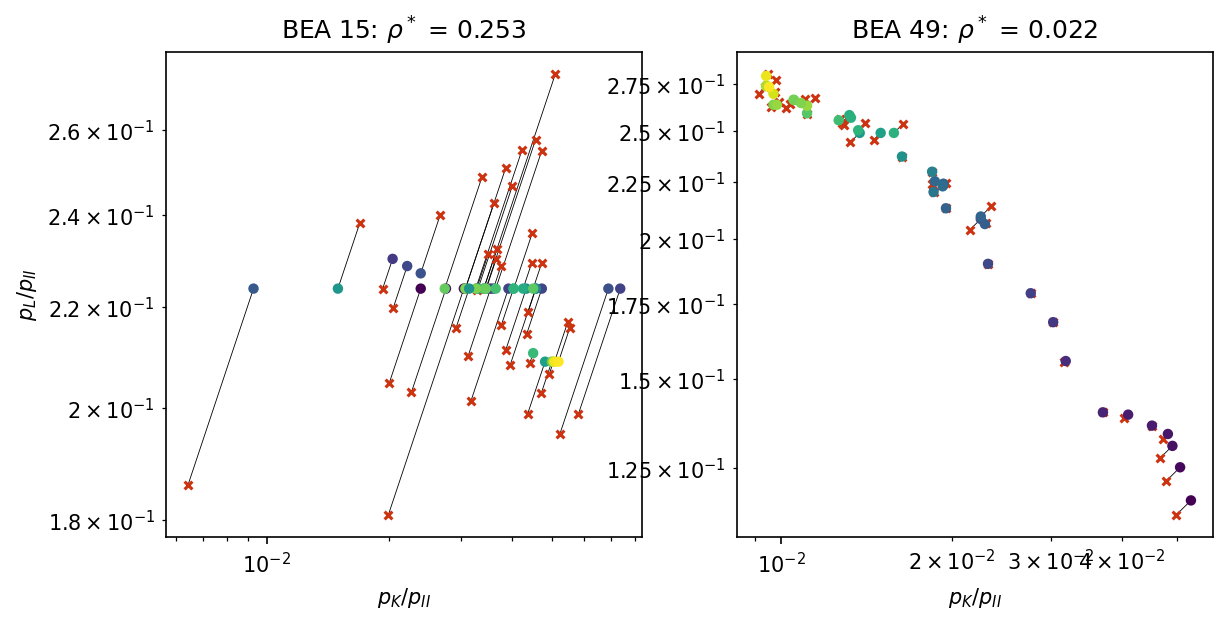
\includegraphics[width=0.85\textwidth]{example_onesided_bea.png}
    \caption{Отрасли BEA, $d=2$. Слева отрасль 15 ($\rho^*/\bar\rho=1$): решение вырождается в прямую $p_L/p_{II}=\mathrm{const}$. Справа отрасль 49 ($\rho^*/\bar\rho=0.05$): вырождения нет.}
\end{figure}

Вырождение профиля в гиперплоскость $p_i=\mathrm{const}$ наблюдается ровно там, где $\rho^*=\bar\rho$. Это наблюдение на четырёх примерах, а не теорема. Содержательно $\rho^*=\bar\rho$ значит, что дешевле всего объяснить данные, лишив одну цену всякой изменчивости.

\section{Эксперименты}

\paragraph{Случайные примеры.} Генератор \texttt{hard\_inst} из тестов. Для каждого примера алгоритм запущен с прямым и обратным порядком приоритета.
\begin{center}
\begin{tabular}{lrrl}
    \toprule
    серия & примеров & ничьих & проверки \\
    \midrule
    $d=2$, $T=4$, точный оракул & 10 & 0 & все пройдены \\
    $d=2$, $T=6$, поток & 30 & 0 & все пройдены \\
    $d=2$, $T=6$, поток, все штрафы равны 1 & 30 & 0 & все пройдены \\
    $d=3$, $T=3$, точный оракул & 15 & 0 & все пройдены \\
    \bottomrule
\end{tabular}
\end{center}
Проверки: $Q$ допустим (коробка $[\theta-2\varepsilon_{\mathrm{low}},\theta+2\varepsilon_{\mathrm{low}}]$ разрешима), все ненулевые единицы блокируют, ни у одного года не ненулевые обе единицы, ответы при двух порядках приоритета совпадают с точностью $10^{-4}$. Ветвь с ничьей проверена на синтетическом монотонном оракуле <<год 0 вверх или год 1 вверх>>.

\paragraph{США, EU KLEMS.} $d=2$, $T=26$, штрафы основного текста. 25 стадий, 1671 обращение, 358 с, ничьих нет. При обратном порядке приоритета 1618 обращений, ответ совпадает точно. С поиском блокирующих единиц делением пополам и запросом только внутренней коробки на стадиях~--- 671 обращение и 120 с, ответ тот же (разница $5\cdot10^{-7}$). Наибольшая поправка $\rho^*=0.05807$ у 2008 года (вверх) и 2020 года (вниз). Величины $\abs{\theta_t}$ совпадают с симметричным профилем во всех 26 годах до шестого знака (1015 обращений, 24 стадии), как и предсказывает теорема~\ref{thm:sym}. Знаки: 1995--2014 вверх, кроме 1996 года, 2015--2020 вниз. Пара 1995 и 1996 исправлена на $\pm0.00404$, то есть разведена в противоположные стороны на одинаковую величину.

\begin{figure}[ht]
    \centering
    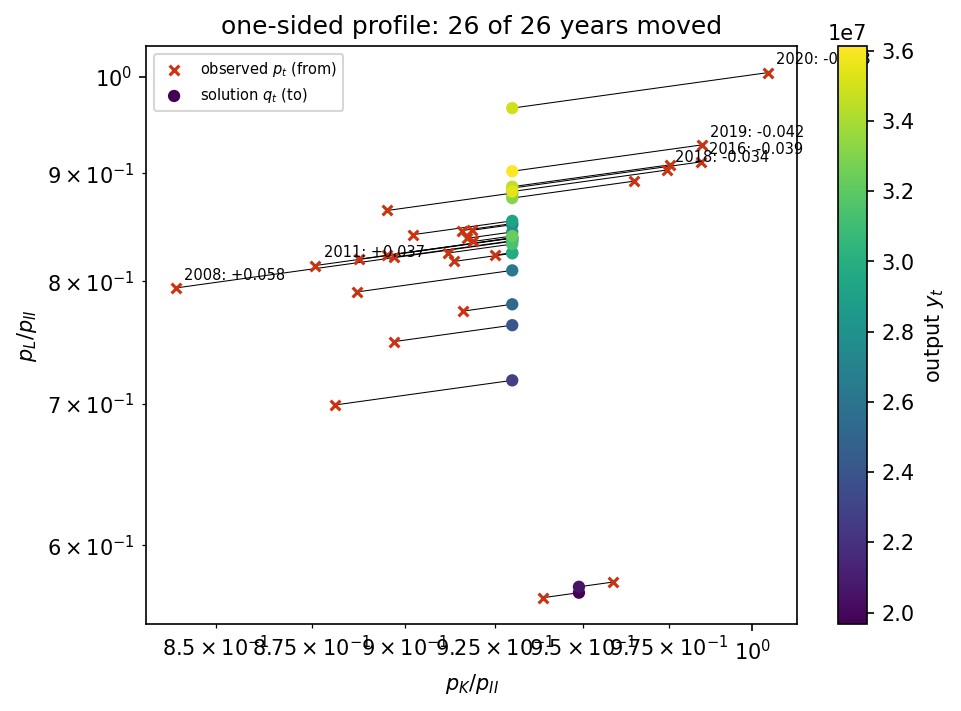
\includegraphics[width=0.62\textwidth]{example_onesided.png}
    \caption{Односторонний профиль, данные США. Крестики~--- наблюдения, точки~--- единственное решение $Q$.}
\end{figure}

\paragraph{США, $d=3$.} Цены K, L, II, нормирующая цена~--- цена выпуска GO, точный оракул. 24 стадии, 663 обращения, 25 мин, ничьих нет, все проверки пройдены. $\rho^*=0.03625$, наибольшие поправки у 2002 года (вверх) и 2018 года (вниз). 2020 год не сдвигается. Знаки: 1995--2004 вверх, с 2005 года в основном вниз (2007--2009 слегка вверх). Разброс $\ln(K/GO)$ уменьшился с $0.046$ до $0.027$, $\ln(II/GO)$ с $0.025$ до $0.015$, $\ln(L/GO)$ почти не изменился. Сингулярные числа облака $\ln Q$ равны $0.63$, $0.15$, $0.048$ против $0.70$, $0.21$, $0.107$ у $\ln P$. Облако сплющивается, но не вырождается ни в плоскость, ни в прямую.

\begin{figure}[ht]
    \centering
    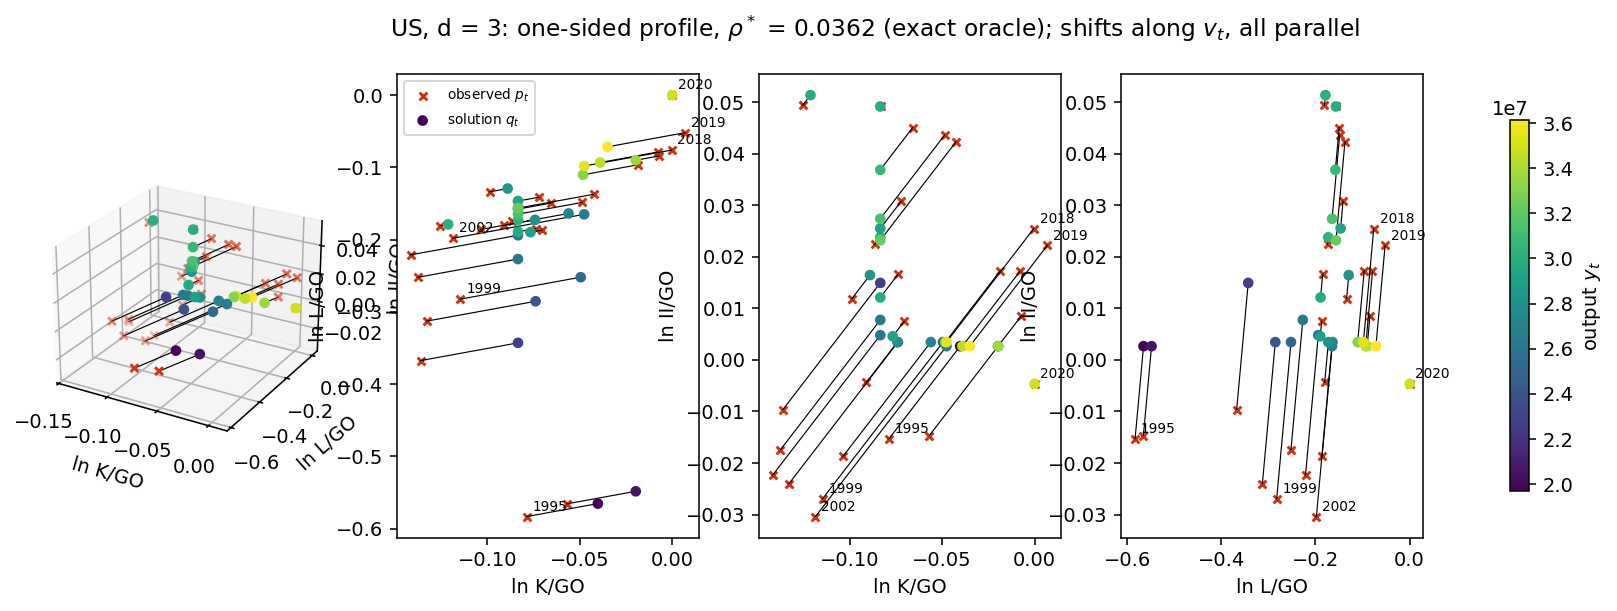
\includegraphics[width=\textwidth]{example_onesided_d3.png}
    \caption{США, $d=3$. Слева трёхмерный вид, справа проекции в координатах $\ln(K/GO)$, $\ln(L/GO)$, $\ln(II/GO)$. Крестики~--- наблюдения, точки~--- решение.}
\end{figure}

\paragraph{Рациональное решение.}

\begin{proposition}[рациональность]\label{prop:rational}
    Пусть рациональные углы $L_t\le U_t$ лежат в шарах $d_{\kappa_t}(\cdot,p_t)\le r_t$ на пути года $t$, причём одна из них равна $p_t$, и пусть задан точный сертификат YES (столбцы и рациональные массы) для коробки $[L,U]$. Тогда существует рациональный набор $Q$ с $d_{\kappa_t}(q_t,p_t)\le r_t$, при котором $y$ слабо разрешим, и он строится по сертификату решением рациональных задач линейного программирования.
\end{proposition}

\begin{proof}
    Возьмём отрезок $z_t(\theta)=L_t+\theta(U_t-L_t)$, $\theta\in[0,1]$, линейный в ценах. Пусть $L_t=p_t$ и $U_t=p_t\circ e^{a}$, $a\ge0$. В логарифмических координатах $x_i(\theta)=\ln\bigl(1+\theta(e^{a_i}-1)\bigr)$, и $\partial x_i/\partial a_i=\theta e^{a_i}/(1+\theta(e^{a_i}-1))\le1$. Поэтому $\abs{x_j-x_i}\le\abs{a_j-a_i}$ и $0\le x\le a$. Точка $x$ с $0\le x_i\le r_t(1/\kappa^i+1/\kappa^0)$ лежит в шаре тогда и только тогда, когда $x_j-x_i\le r_t(1/\kappa^i+1/\kappa^j)$ при всех $i,j$: нужно $s\in[-r_t/\kappa^0,r_t/\kappa^0]$ с $\abs{x_i+s}\le r_t/\kappa^i$. Для точек пути $\abs{a_j-a_i}\le r_t\abs{1/\kappa^j-1/\kappa^i}$, поэтому отрезок лежит в шаре. Случай $U_t=p_t$ симметричен.

    Доказательство (C)$\Rightarrow$(B) теоремы об углах использует только непрерывный монотонный путь между углами. Для отрезка точка входа $\gamma_{k,t}=\min\set{\theta\in[0,1]\mid z_t(\theta)\in K_k}$ есть значение рациональной задачи линейного программирования. Выбранное $\theta_t$ равно $0$, $1$ или одному из $\gamma_{k,t}$, поэтому $q_t=z_t(\theta_t)$ рационально.
\end{proof}

В коде (\texttt{onesided.rational\_solution}) сначала проверяется набор из округлённых внутрь углов. Округлённый угол лежит в шаре, так как у вершины зонотоп локально совпадает с <<вершина минус положительный ортант>>. Если проверка не проходит, применяется построение утверждения~\ref{prop:rational}. На данных США при $d=3$ прошла уже проверка углов, сертификат состоит из 26 множеств. Построение по отрезку проверено тестами при $d=2$ и $d=3$.

\section{Размерность и агрегация}

\paragraph{Откуда берутся малые $d$.} В данных BEA для каждой отрасли и года есть девять цен: пять типов капитала, два типа труда, промежуточные затраты II и цена выпуска GO. Выпуск $y$~--- индекс количества валового выпуска GO\_Q во всех вариантах. Варианты различаются набором цен и нормирующей ценой.
\begin{center}
\begin{tabular}{lll}
    \toprule
    вариант & цены & нормирующая цена \\
    \midrule
    $d=2$ & K, L (индексы Торнквиста) & II, цены выпуска нет \\
    $d=3$ & K, L, II & GO \\
    $d=4$ & K, два типа труда, II & GO \\
    $d=7$ & пять типов капитала, два типа труда & II, цены выпуска нет \\
    $d=8$ & пять типов капитала, два типа труда, II & GO \\
    \bottomrule
\end{tabular}
\end{center}
Полная задача~--- $d=8$. Варианты $d=2$ и $d=7$ отбрасывают цену выпуска.

\paragraph{Механический эффект.} Пусть нормирующая цена та же. Если отбросить координату, свидетель с нулём в этой координате годится и в полной задаче. Поэтому при фиксированных ценах семейство слабо достижимых множеств в задаче меньшей размерности не больше, чем в полной. Больше координат~--- слабее проверка, и $\rho^*$ падает уже поэтому. Агрегация не является проекцией, и для неё такого вложения в общем случае нет.

\paragraph{Контроль.} Для каждого типа капитала и труда отклонения $\ln p_{k,t}-\ln p_{K,t}$ от агрегата переставлены по годам случайно. Размер детализации сохраняется, связь с годами разрушается. Наименьший уровень $\rho^*$ найден точным оракулом.
\begin{center}
\begin{tabular}{lrrrr}
    \toprule
    отрасль BEA & $d=2$ & $d=3$ & $d=8$ & $d=8$, контроль \\
    \midrule
    15 Motor vehicles & 0.253 & 0.099 & 0.0057 & 0.093, 0.076 \\
    24 Petroleum & 0.473 & 0.157 & 0.018 & 0.137, 0.117 \\
    1 Farms & 0.229 & 0.241 & 0.038 & 0.180, 0.202 \\
    6 Utilities & 0.199 & 0.053 & 0.043 & \\
    12 Machinery & 0.039 & 0.051 & 0.033 & \\
    27 Wholesale trade & 0.054 & 0.072 & 0.024 & \\
    31 Water transportation & 0.045 & 0.130 & 0.036 & \\
    46 Rental and leasing & 0.020 & 0.016 & 0.0025 & \\
    49 Prof.\ services & 0.022 & 0.013 & 0.0098 & \\
    63 State and local & 0.153 & 0 & 0 & \\
    \bottomrule
\end{tabular}
\end{center}
Отношения $\rho^*/\bar\rho$ при $d=3$: 15~--- 0.81, 1~--- 0.68, 6~--- 0.36, 12~--- 0.63, 24~--- 0.75, 27~--- 0.93, 31~--- 0.42, 46~--- 0.19, 49~--- 0.15, 63~--- 0. Вырожденных случаев при $d\ge3$ нет.

Настоящая детализация уменьшает $\rho^*$ в 5--17 раз, контрольная~--- на 5--25\%. Значит, падение не механическое: индексы Торнквиста теряют информацию, которую использует модель. Цена выпуска в роли нормирующей снимает вырождение уже при $d=3$: у отрасли 15 отношение $\rho^*/\bar\rho$ падает с $1.00$ до $0.81$. Детализация помогает не везде. У отрасли 6 $\rho^*$ при $d=4$ и $d=8$ одинаков, у отраслей 12, 24, 46 одинаковы $d=3$ и $d=4$. Контроль сделан на трёх отраслях по две перестановки.

\section{Интерпретация}

\paragraph{Поправка как ошибка измерения.} Сдвиг года $t$ на $\theta_t$ вдоль пути означает поправки логарифмов измеренных цен $\delta^i_t=\theta_t/\kappa^i_t$ при $i\ge1$ и $\delta^0_t=-\theta_t/\kappa^0_t$. Это разложение сдвига с наименьшим наибольшим взвешенным отклонением $\kappa\abs\delta$, и оно равно $\abs{\theta_t}$. При $\theta_t>0$ цены $1,\dots,d$ года $t$ измерены заниженными относительно нормирующей цены, при $\theta_t<0$ завышенными. Цены с малым штрафом получают большую долю поправки.

\paragraph{Обратная задача.} Модель ошибок здесь множественная (bounded error, set-membership): ошибка цены $i$ года $t$ не больше $\rho/\kappa^i_t$ с неизвестным общим $\rho$. Число $\rho^*$~--- наименьший уровень ошибок, совместимый с моделью. Множество совместимых $Q$ при $\rho^*$ обычно не точка, и нужно правило выбора, как минимальная норма при регуляризации Тихонова. Лексикографический профиль есть такое правило в той же метрике $\ell^\infty$. Сначала минимизируется наибольшая ошибка, затем следующая и так далее. В выпуклых задачах чебышёвского приближения это строгое чебышёвское приближение. Оно единственно и является пределом $\ell^p$-приближений при $p\to\infty$. Здесь множество невыпукло, и теорема о пределе не доказана. Единственность $Q$ доказана напрямую (теорема~\ref{thm:unique}).

\paragraph{Каждая поправка необходима.} Ненулевая поправка блокирует: её нельзя уменьшить, не увеличив поправки других лет. Это проверяемо, отказ оракула при уменьшенной поправке служит сертификатом. Знак поправки однозначен. Ни один год не исправлен сильнее, чем нужно при уже исправленных годах с большими поправками. Это аналог нуклеолуса: бремя исправления распределяется между годами от наибольшего к наименьшему.

\paragraph{Ограничения.} Правило чебышёвское и распределяет поправку по многим годам: в данных США двигаются все 26 лет. Оно подходит для малых ошибок во всех данных (дефляторы, вменённая цена капитала). Оно не подходит для модели с немногими грубыми выбросами. Там нужна разреженная поправка, то есть наименьшее число исправленных лет или наименьшая сумма поправок. По разделу о суммах в модели с оракулом это требует экспоненциально много запросов. В теории выявленных предпочтений аналогичные индексы на наблюдение также трудны. Правило также не вероятностное: оно не оценка максимального правдоподобия и не даёт доверительных интервалов. При ничьей выбор зависит от порядка приоритета. Естественный порядок~--- априорная надёжность лет.

\begin{remark}[литература, ссылки не проверены]
    Строгое чебышёвское приближение: J.~R.~Rice (1962), J.~Descloux (1963). Наименьшие поправки данных до согласия с оптимизирующим поведением: H.~Varian (1985, 1990), индекс Африата, индекс Houtman--Maks. Трудность индекса Varian на наблюдение: Smeulders, Spieksma, Cherchye, De Rock (2014). Нуклеолус: D.~Schmeidler (1969).
\end{remark}

\section{Открытые вопросы}

\begin{enumerate}
    \item Общность положения. Доказать, что при штрафах вне множества меры нуль ничьих нет и профиль единственен без приоритета. Вероятный путь: уровни стадий суть корни экспоненциальных сумм из теоремы о точках излома, и совпадение двух уровней задаёт условие коразмерности один на штрафы.
    \item Оценка погрешности по стадиям при конечной точности бисекции.
    \item Решения вне путей на гранях через дальний угол (утверждение~\ref{prop:offpath}). Либо доказать, что их нет, либо уточнить единицы до односторонних ошибок отдельных цен $(t,i,\pm)$, $i=0,\dots,d$. Запрос тогда остаётся одним: коробка $p^i_te^{-(\alpha^i_t+\beta^0_t)}\le q^i_t\le p^i_te^{\beta^i_t+\alpha^0_t}$. Но блокировка прижимает $q_t$ к грани, а не к точке, и доказательство единственности не переносится.
    \item Вырождение профиля в гиперплоскость $p_i=\mathrm{const}$ ровно при $\rho^*=\bar\rho$: доказать или опровергнуть.
    \item Контроль агрегации на всех отраслях и с большим числом перестановок.
    \item Lean: леммы~\ref{lem:block}, \ref{lem:pareto}, \ref{lem:cover}, теоремы~\ref{thm:unique}, \ref{thm:sym}, утверждение~\ref{prop:rational}. Лемма~\ref{lem:corners} требует обобщить \texttt{wfeasible\_iff\_path} на несимметричные отрезки.
\end{enumerate}

Код: \texttt{perturb/onesided.py}, \texttt{perturb/exact\_oracle.py}. Примеры: \texttt{experiments/us\_onesided.py}, \texttt{us\_onesided\_d3.py}, \texttt{bea\_onesided.py}, \texttt{ratio\_d3.py}, \texttt{aggregation.py}, логи в \texttt{experiments/results/}. Тесты: \texttt{tests/test\_onesided.py}, \texttt{tests/test\_exact\_oracle.py}.

\end{document}
